%%This is a very basic article template.
%%There is just one section and two subsections.
\documentclass{article}

\usepackage{cite}
\usepackage{graphicx}

\begin{document}
\title{Self Consistent Inverse Pronlem With Cross Validation}
\maketitle

\section{Introduction and Motivation}
The mathematical term well-posed problem stems from a definition given by
Jacques Hdamard. He believed that mathematical models of physical phenomena
should have the properties that.
\begin{enumerate} 
  \item A solution exists.
  \item The solution is unique.
  \item The solution's behavior changes continuously with the initial
  conditions.
\end{enumerate}
Problems that are not well-posed in the sense
of Hadamard are termed ill-posed. Inverse problems are often ill-posed.

Continuum models must often be discretized in order to obtain a numerical
solution, while solutions may be continuous with respect to the initial
conditions, they may suffer from numerical instability when solved with finite
precision, or with erros in the data. Even if a problem is well posed, it may
still be ill-conditioned, meaning that a small error in the intial data can
result in much larger errors in the answers.

In order to solve the ill-posed problem, regularization method is introduced. A
simple form of regularization applied to integral equations, generally termed
Tikhonov regularization, is essentially a trade-off between fitting the data and
reducing a norm of the solution. 

Ill-posed inverse problem with the regularization method can give out a very
good reconstructed result compared to the exact result, but only if the measured
value and the model is accurate enough.

In order to solve the ill-posed inverse problem which the measure value or the 
model is not accurate enougth to give out a good reconstructed result, we
introduce the self consistent regularization method With Cross Validation.


\section{Generalized Cross Validation}
The fitness is calculated as:
\begin{equation}
	\mathop {\min }\limits_\lambda  ||A{x_\lambda } - {b^{exact}}||_2^2
\end{equation}

However, we can't calculate it since \(b^{exact}\) is not available. Generalized 
Cross Validation is a classical statistical technique that comes into good use
here \cite{hansen2010discrete}.

Using Generalized Cross Validation(GSV), the fitness can be calculated as:
\begin{equation}
	\mathop {\min }\limits_\lambda  \frac{{||A{x_\lambda } - b||_2^2}}{{{{(m -
	\sum\nolimits_{i = 1}^n {\varphi _i^{[\lambda ]}} )}^2}}}
\end{equation}

\section{Cellular Evolutionary Algorithm}
Usually EAs assume that the strucutre of the population is panmictic, which
means that any inidividual may interact with any other individual in the
population.
However, this need not be always the case: we often see population sin the
biological and social world in which individuals only interact with a subset of
the rest of the population. This situation can usefully be depicated by using
the concept of a population graph \cite{hoekstra2010simulating}.

\section{Result}
\begin{figure}[h!]
  \centering
    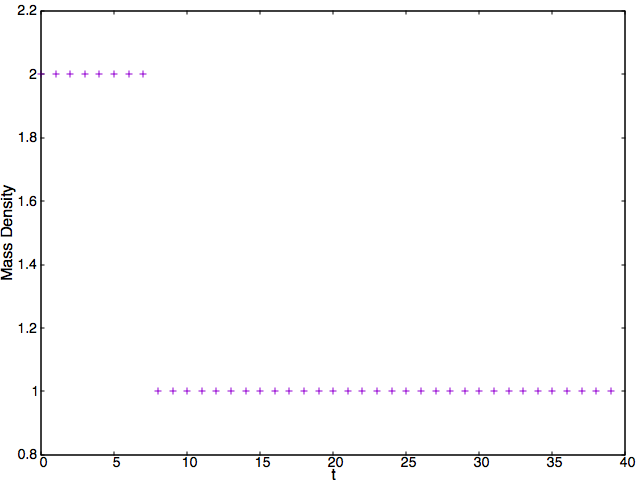
\includegraphics[width=0.7\textwidth]{images/exactmassdensity}
  \caption{Exact f function (mass density distribution)}
  \label{fig:MASS}
\end{figure}
\begin{figure}[h!]
  \centering
    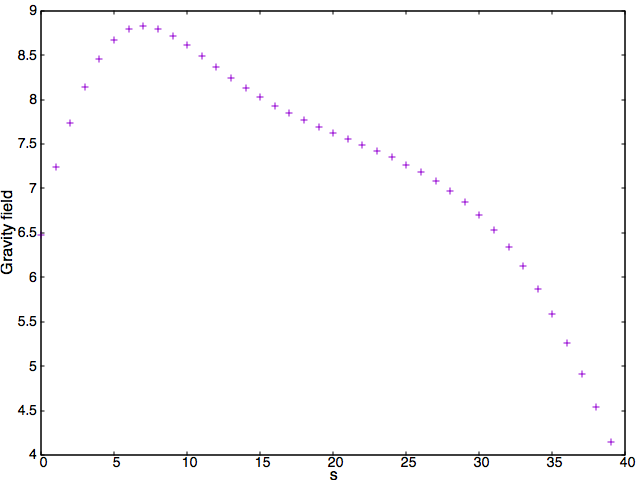
\includegraphics[width=0.7\textwidth]{images/exactgravityfield}
  \caption{Exact signal g (the gravity field)}
  \label{fig:G}
\end{figure}
\begin{figure}[h!]
  \centering
    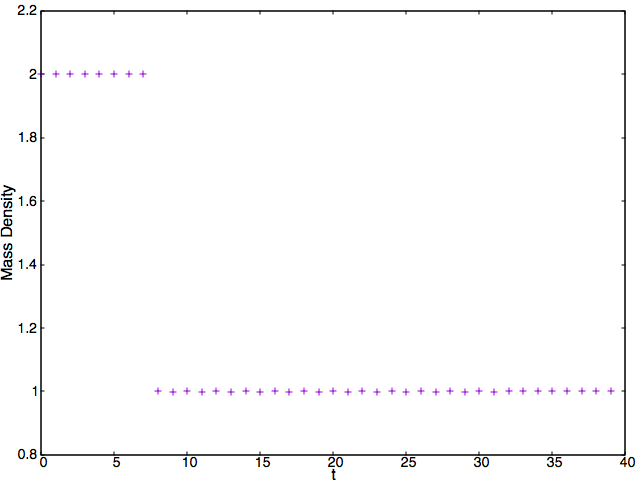
\includegraphics[width=0.7\textwidth]{images/reconstructedmassdensitygood}
  \caption{The Reconstructed function f(the mass density distribution) after
  self-consistent genetic algorithm, at \(\lambda  = {10^{ - 12}}\), GSV value
  = 1.65e-25}
  \label{fig:RMASSGOOD}
\end{figure}
\begin{figure}[h!]
  \centering
    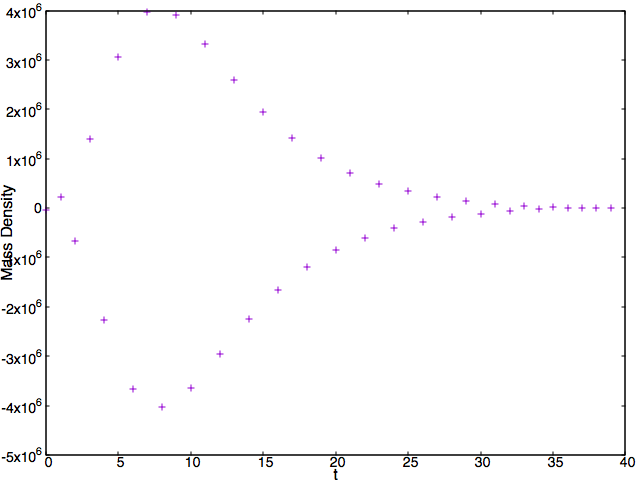
\includegraphics[width=0.7\textwidth]{images/reconstructedmassdensitybad}
  \caption{The Reconstructed function f(the mass density distribution) without
  self-consistent genetic algorithm, at \(\lambda  = {10^{ - 12}}\), GSV value
  = 7.22e-10}
  \label{fig:RMASSBAD}
\end{figure}

\bibliography{mybib}{}
\bibliographystyle{plain}
\end{document}
